%%%%%%%%%%%%%%%%%%%%%%%%%%%%%%%%%%%%%%%%%
% Beamer Presentation
% LaTeX Template
% Version 1.0 (10/11/12)
%
% This template has been downloaded from:
% http://www.LaTeXTemplates.com
%
% License:
% CC BY-NC-SA 3.0 (http://creativecommons.org/licenses/by-nc-sa/3.0/)
%
%%%%%%%%%%%%%%%%%%%%%%%%%%%%%%%%%%%%%%%%%

%----------------------------------------------------------------------------------------
%	PACKAGES AND THEMES
%----------------------------------------------------------------------------------------

\PassOptionsToPackage{table,xcdraw}{xcolor}

\documentclass{beamer}

\mode<presentation> {

% The Beamer class comes with a number of default slide themes
% which change the colors and layouts of slides. Below this is a list
% of all the themes, uncomment each in turn to see what they look like.

%\usetheme{default}
%\usetheme{AnnArbor}
%\usetheme{Antibes}
%\usetheme{Bergen}
%\usetheme{Berkeley}
%\usetheme{Berlin}
%\usetheme{Boadilla}
\usetheme{CambridgeUS}
%\usetheme{Copenhagen}
%\usetheme{Darmstadt}
%\usetheme{Dresden}
%\usetheme{Frankfurt}
%\usetheme{Goettingen}
%\usetheme{Hannover}
%\usetheme{Ilmenau}
%\usetheme{JuanLesPins}
%\usetheme{Luebeck}
%\usetheme{Madrid}
%\usetheme{Malmoe}
%\usetheme{Marburg}
%\usetheme{Montpellier}
%\usetheme{PaloAlto}
%\usetheme{Pittsburgh}
%\usetheme{Rochester}
%\usetheme{Singapore}
%\usetheme{Szeged}
%\usetheme{Warsaw}

% As well as themes, the Beamer class has a number of color themes
% for any slide theme. Uncomment each of these in turn to see how it
% changes the colors of your current slide theme.

%\usecolortheme{albatross}
%\usecolortheme{beaver}
%\usecolortheme{beetle}
%\usecolortheme{crane}
%\usecolortheme{dolphin}
%\usecolortheme{dove}
%\usecolortheme{fly}
%\usecolortheme{lily}
%\usecolortheme{orchid}
%\usecolortheme{rose}
%\usecolortheme{seagull}
%\usecolortheme{seahorse}
%\usecolortheme{whale}
%\usecolortheme{wolverine}

%\setbeamertemplate{footline} % To remove the footer line in all slides uncomment this line
%\setbeamertemplate{footline}[page number] % To replace the footer line in all slides with a simple slide count uncomment this line

%\setbeamertemplate{navigation symbols}{} % To remove the navigation symbols from the bottom of all slides uncomment this line

\definecolor{naranja}{RGB}{255,192,0} % changed this
\definecolor{verde}{RGB}{0,128,0} % changed this

\setbeamercolor{title}{fg=white,bg=black} % changed this
\setbeamercolor{author}{fg=black,bg=gray!25} % changed this
\setbeamercolor{institute}{fg=black,bg=white} % changed this
\setbeamercolor{frametitle}{fg=black,bg=white} % changed this

\setbeamercolor{block title}{fg=white,bg=naranja}
\setbeamercolor{block body}{fg=black,bg=gray!25}

\setbeamercolor{block title example}{fg=white,bg=verde}
\setbeamercolor{block body example}{fg=black,bg=gray!25}

\setbeamercolor{palette primary}{fg=white,bg=black} % changed this
\setbeamercolor{palette secondary}{fg=black,bg=gray!25} % changed this
\setbeamercolor{palette tertiary}{fg=black,bg=naranja} % changed this
\setbeamercolor{palette quaternary}{fg=black,bg=white} % changed this

%\setbeamertemplate{background}{\includegraphics[width=1.15\textwidth]{IMG_4705a.jpg}}
}

\usepackage[spanish,es-tabla]{babel}
\usepackage[utf8]{inputenc}
\usepackage{graphicx} % Allows including images
\usepackage{booktabs} % Allows the use of \toprule, \midrule and \bottomrule in tables

\usepackage{amsmath,amssymb,latexsym}

\usepackage{hyperref}

\usepackage{booktabs,colortbl}


\setlength{\arrayrulewidth}{0.5mm}

\renewcommand{\baselinestretch}{1.0}

\hypersetup{
    %hidelinks=blue,         % show bookmarks bar?
    %colorlinks=true,        % false: boxed links; true: colored links
    %linkcolor=white,        % color of internal links (change box color with linkbordercolor)
    citecolor=green,        % color of links to bibliography
    filecolor=magenta,      % color of file links
    urlcolor=blue           % color of external links
}

\usepackage{textpos}

%----------------------------------------------------------------------------------------
%	TITLE PAGE
%----------------------------------------------------------------------------------------

\title[]{\textbf{Implementación automatizada de redes neuronales para sistemas embebidos}} % 
\subtitle{\textbf{Plan de trabajo proyecto especialización en sistemas embebidos}} %The short title appears at the bottom of every slide, the full title is only on the title page

\author[]{Autor: Ing. Jose David Alvarado Moreno  \\ \and  Director: Ing. Federico G. Zacchigna} % Your name
%\institute[USB BOG] % Your institution as it will appear on the bottom of every slide, may be shorthand to save space

%\inst{\S} \\ \inst{\S}

%\author{José David Alvarado Moreno}  
%\author{Federico G. Zacchigna}  

\institute[]{
				
				
\includegraphics[scale=0.05]{Figuras/logoFIUBA}										
}

%\logo{\includegraphics[scale=0.2]{Logos-USB_Sede_Bogota-Vertica_Letra_blanca.png}}

\date{}

\usepackage{svg}

\usepackage[document]{ragged2e}

\renewcommand{\baselinestretch}{1.0}

\usepackage{pgfgantt}

% Activity On Node

\usepackage[table]{xcolor}
\usepackage{pgfplots}
\usepackage{array}

\definecolor{mygray}{RGB}{231,236,240}
\definecolor{myorange}{RGB}{253,205,148}
\definecolor{myblue}{RGB}{107,146,201}

\newcommand\ActTable[7]{%
  \begingroup
  \sffamily
  \renewcommand\arraystretch{1.5}%
  \begin{tabular}{*{3}{|>{\centering\arraybackslash}p{0.5cm}}|}
  \hline
  \rowcolor{mygray} #2 & #3 & #4 \\
  \hline
  \rowcolor{mygray}\multicolumn{3}{|c|}{#1} \\
  \hline
  \cellcolor{mygray}#5 & \cellcolor{myorange}\bfseries#6 & \cellcolor{mygray}#7 \\
  \hline
  \end{tabular}%
  \endgroup
}

\newcolumntype{M}[1]{>{\centering\arraybackslash}m{#1}}

\begin{document}

\begin{frame}
\titlepage % Print the title page as the first slide
\end{frame}

%\logo{\includegraphics[scale=0.05]{Logo_USB_Sede-Bogota-Vertical.png}\hspace{320pt}\vspace{250pt}}

\author{José David Alvarado Moreno}  
\title{Plan de trabajo proyecto} % 
\date{Esp. sistemas embebidos} % Date, can be changed to a custom date

\addtobeamertemplate{frametitle}{}{%
\begin{textblock*}{100mm}(.87\textwidth,-0.8cm)

\includegraphics[scale=0.02]{Figuras/logoFIUBA} 
\end{textblock*}}
											
\setbeamertemplate{background}{}

\begin{frame}
\frametitle{Contenido} % Table of contents slide, comment this block out to remove it
\tableofcontents % Throughout your presentation, if you choose to use \section{} and \subsection{} commands, these will automatically be printed on this slide as an overview of your presentation
\end{frame}

%----------------------------------------------------------------------------------------
%	PRESENTATION SLIDES
%----------------------------------------------------------------------------------------

%------------------------------------------------
\section{Descripción}
%------------------------------------------------

\begin{frame}[allowframebreaks,c]

\frametitle{Descripción}

\centering

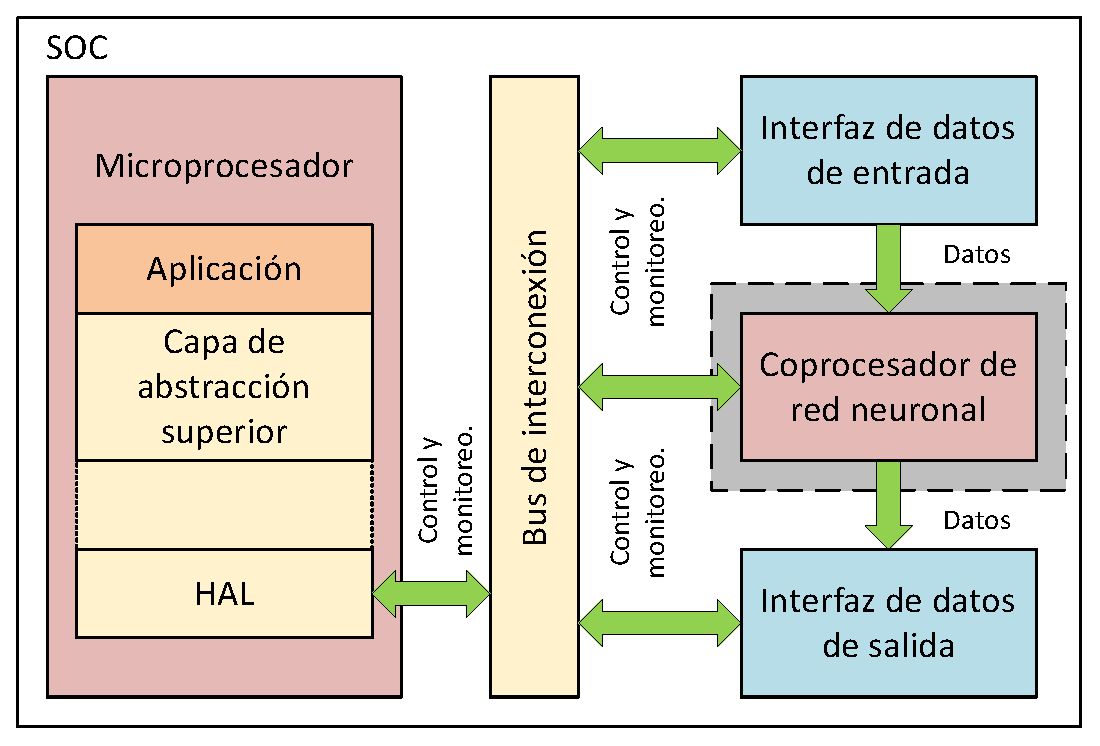
\includegraphics[scale=0.5]{Figuras/Diagramas}

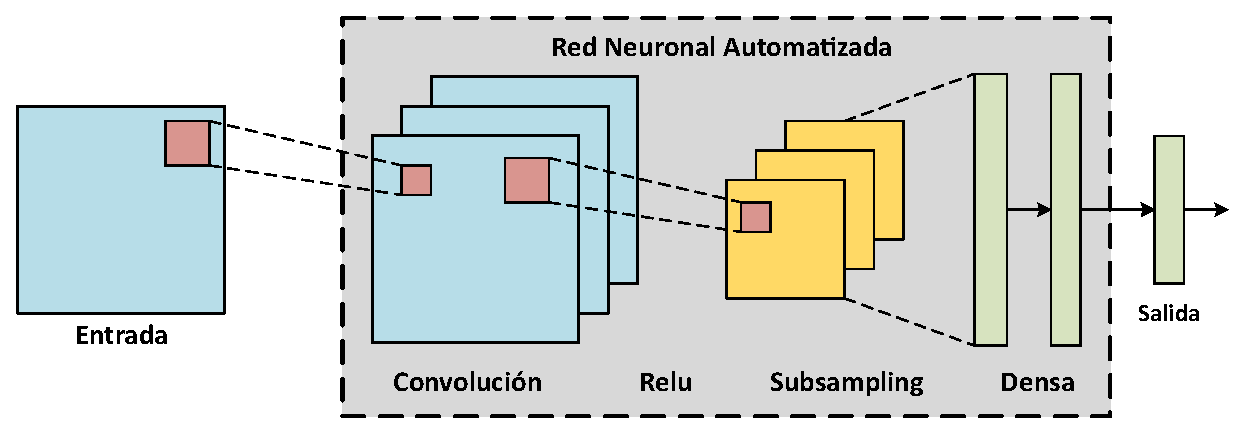
\includegraphics[scale=0.55]{Figuras/RN1}

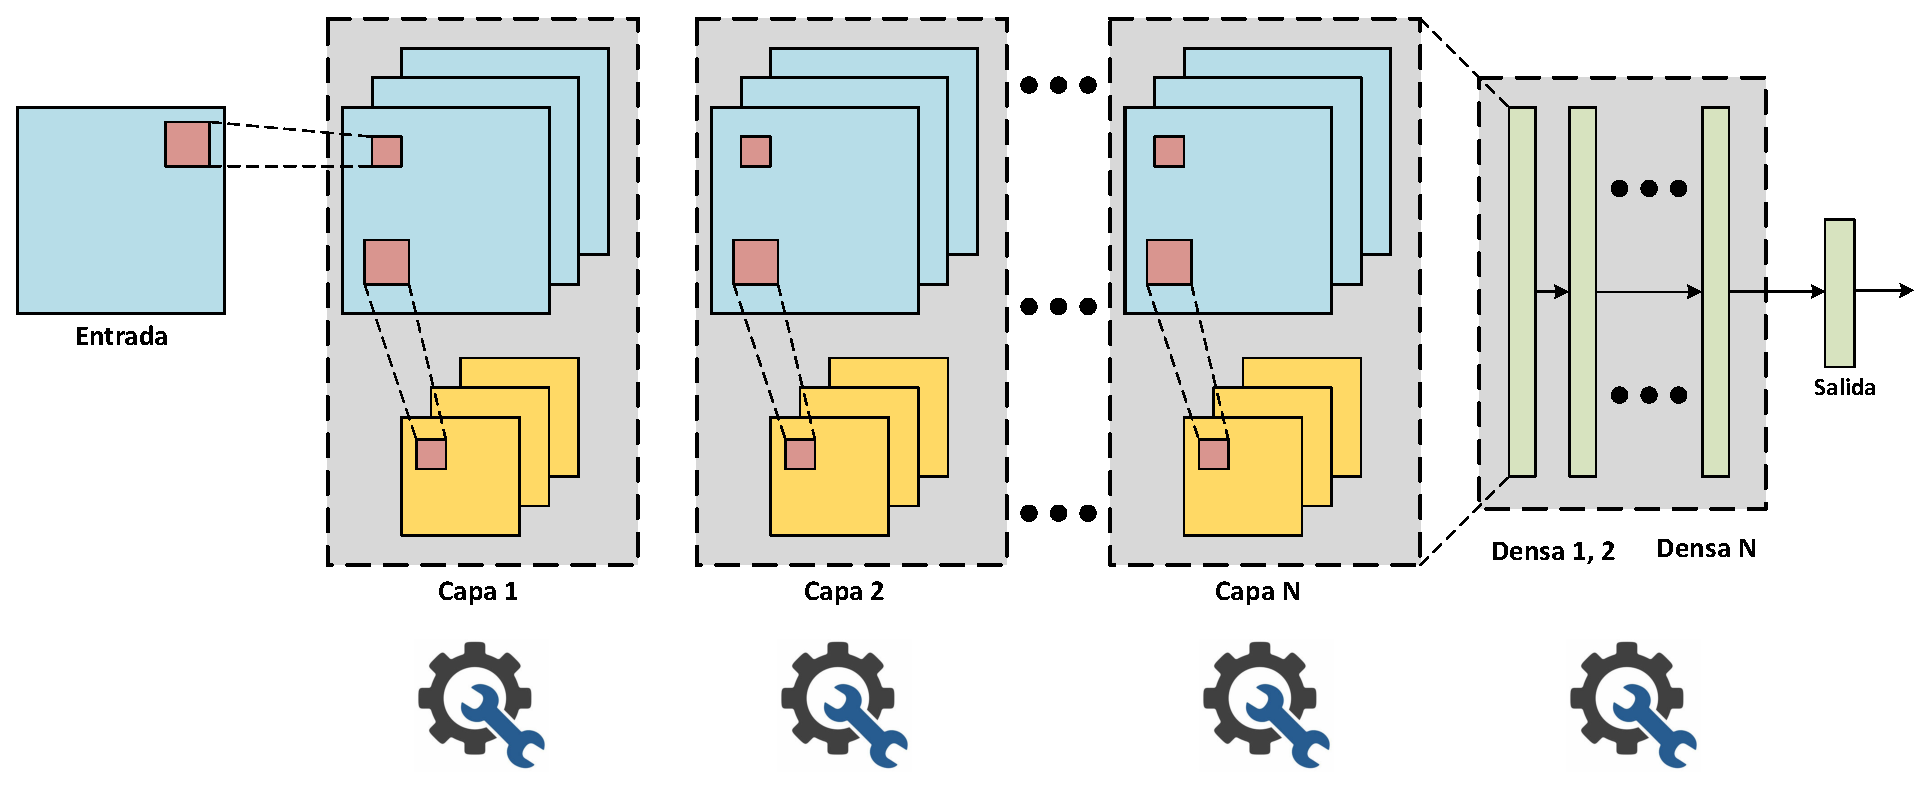
\includegraphics[scale=0.35]{Figuras/RN2}

\justifying

\vspace{0.5cm}

Parámetros: Tamaño de los datos de entrada, números de capas, valores de los pesos de la red neuronal, seleccionar métodos de activación.  

\end{frame}

%------------------------------------------------
\section{Interesados}
%------------------------------------------------

\begin{frame}[allowframebreaks,c]

\frametitle{Interesados}

\centering


\includegraphics[scale=0.45]{Figuras/INT}

\end{frame}

%------------------------------------------------
\section{Propósito del proyecto}
%------------------------------------------------

\begin{frame}[allowframebreaks,t]

\frametitle{Propósito del proyecto}

\justifying

Con este proyecto se busca realizar un \textbf{coprocesador automatizado} para redes neuronales utilizando un \textbf{sistema embebido} compuesto por \textbf{SoC-FPGA}. \\

\centering

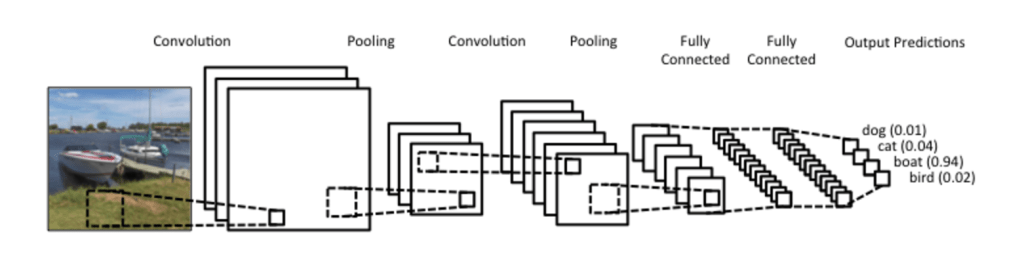
\includegraphics[scale=0.26]{Figuras/AP1} \\\
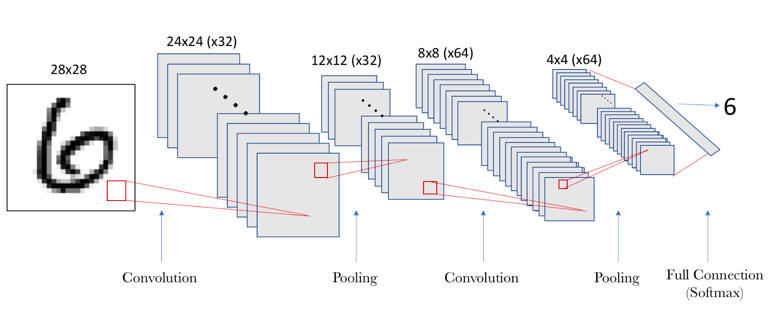
\includegraphics[scale=0.26]{Figuras/AP2}

\end{frame}

%------------------------------------------------
\section{Alcances del proyecto}
%------------------------------------------------

\begin{frame}[allowframebreaks,t]

\frametitle{Alcances del proyecto}

\justifying

\textbf{Incluye:} \\\

\begin{itemize}
	\item Un sistema para general el \textbf{modelo de alto nivel} de red neuronal utilizando una herramienta de software especializada (Keras).    
	\item Un \textbf{coprocesador} de redes neuronales convolucionales automatizadas.
	\item Reportes de los \textbf{resultados de validación} del sistema.
\end{itemize}

\vspace{0.5cm}

\textbf{No incluye:} \\\

El presente proyecto no incluye realizar procesos de optimización, no se utilizaran dispositivos adicionales a la FPGA \textbf{PYNQ-Z2}.

\end{frame}

%------------------------------------------------
\section{Requerimientos del proyecto}
%------------------------------------------------

\begin{frame}[allowframebreaks,t]

\frametitle{Requerimientos del proyecto}

\Large 

Modelo de alto nivel.  						\\ \vspace{0.3cm}
Cuantización. 										\\ \vspace{0.3cm}
Arquitectura de alto nivel. 			\\ \vspace{0.3cm}
Micro-arquitectura. 							\\ \vspace{0.3cm}
Integración de HW-SW. 						\\ \vspace{0.3cm}
Verificación y validación. 				


\end{frame}
%------------------------------------------------
\section{Diagrama actividades}
%------------------------------------------------

\begin{frame}[allowframebreaks,c]

\frametitle{Diagrama actividades}

\vspace{0.5cm}

\resizebox{.45\textwidth}{!}{
\begin{picture}(210,260)(0,-30)

% Inicio

\put(50,200){\oval(60,40)}
\put(36,198){\textbf{Inicio}}

% Columna 1

\put(110,200){\ActTable{Planificación}{1}{3}{3}{1}{3}{6}}

\put(110,120){\ActTable{Revisión}{1}{6}{6}{1}{0}{6}}

% Columna 2

\put(220,200){\ActTable{Desarrollo}{7}{16}{22}{7}{0}{22}}

% Columna 3

\put(330,200){\ActTable{Verificación}{23}{4}{26}{23}{0}{26}}


\put(330,40){\ActTable{Cierre}{27}{6}{32}{27}{0}{32}}

% Fin

\put(50,40){\oval(60,40)}
\put(42,38){\textbf{Fin}}

%% The arrrows 

\thicklines
\color{myblue}

\put(80,200){\vector(1,0){30}}
\put(90,200){\line(0,-1){80}}
\put(90,120){\vector(1,0){20}}

\put(190,200){\vector(1,0){30}}
\put(205,200){\line(0,-1){80}}
\put(190,120){\line(1,0){15}}

\put(300,200){\vector(1,0){30}}

\put(410,200){\line(1,0){15}}
\put(425,200){\line(0,-1){160}}
\put(425,40){\vector(-1,0){15}}

\put(330,40){\vector(-1,0){250}}

\end{picture}
}


\end{frame}
%------------------------------------------------
\section{Diagrama de Gantt}
%------------------------------------------------

\begin{frame}[allowframebreaks,c]

\frametitle{Diagrama de Gantt}


\definecolor{barblue}{RGB}{153,204,254}
\definecolor{groupblue}{RGB}{51,102,254}
\definecolor{linkred}{RGB}{165,0,33}
\renewcommand\sfdefault{phv}
\renewcommand\mddefault{mc}
\renewcommand\bfdefault{bc}
\setganttlinklabel{s-s}{}%{START-TO-START}
\setganttlinklabel{f-s}{}%{FINISH-TO-START}
\setganttlinklabel{f-f}{}%{FINISH-TO-FINISH}
\sffamily

\begin{ganttchart}[x unit=0.29cm, y unit chart =0.9cm,
    canvas/.append style={fill=none, draw=black!5, line width=.75pt},
    hgrid style/.style={draw=black!5, line width=.75pt},
    vgrid={*1{draw=black!5, line width=.75pt}},
    %today=7, today rule/.style={ draw=black!64, dash pattern=on 3.5pt off 4.5pt, line width=1.5pt},
    %today label font=\small\bfseries,
    title/.style={draw=none, fill=none},
    title label font=\bfseries\footnotesize,
		title label node/.append style={below=6pt},
    include title in canvas=false,
    bar label font=\mdseries\small\color{black!70},
    %bar label node/.append style={left=0cm},
    bar/.append style={draw=none, fill=black!63},
    bar incomplete/.append style={fill=barblue},
    bar progress label font=\mdseries\footnotesize\color{white},
    group incomplete/.append style={fill=groupblue},
    group left shift=0,
    group right shift=0,
    group height=.5,
    group peaks tip position=0,
    group label node/.append style={left=.6cm},
    group progress label font=\bfseries\small\color{white},
    link/.style={-latex, line width=0.5pt, linkred},
    link label font=\scriptsize\bfseries,
    link label node/.append style={below left=-2pt and 0pt}
  ]{1}{32}
  \gantttitle[ title label node/.append style={below left=7pt and -3pt}]{Semana:\quad1}{1}
  \gantttitlelist{2,,4,,6,,8,,10,,12,,14,,16,,18,,20,,22,,24,,26,,28,,30,,32}{1} \\
  \ganttgroup[progress=80]{Planificación}{1}{2} \\
  %\ganttbar[progress=80, name=EDT11]{\textbf{EDT 1.1} }{1}{1} \\
  %\ganttbar[progress=80, name=EDT12]{\textbf{EDT 1.2} }{2}{2} \\ 	[grid]
  
	\ganttgroup[progress=0]{Revisión}{3}{6} \\
  %\ganttbar[progress=0, name=EDT21]{\textbf{EDT 2.1} }{3}{4} \\
  %\ganttbar[progress=0, name=EDT22]{\textbf{EDT 2.2} }{5}{5} \\
  %\ganttbar[progress=0, name=EDT23]{\textbf{EDT 2.3} }{6}{6} \\	[grid]
  
	\ganttgroup[progress=0]{Desarrollo}{7}{22} \\
  %\ganttbar[progress=0, name=EDT31]{\textbf{EDT 3.1} }{7}{8} \\
  %\ganttbar[progress=0, name=EDT32]{\textbf{EDT 3.2} }{9}{11} \\
  %\ganttbar[progress=0, name=EDT33]{\textbf{EDT 3.3} }{12}{13} \\
  %\ganttbar[progress=0, name=EDT34]{\textbf{EDT 3.4} }{14}{16} \\
	%\ganttbar[progress=0, name=EDT35]{\textbf{EDT 3.5} }{17}{19} \\
  %\ganttbar[progress=0, name=EDT36]{\textbf{EDT 3.6} }{20}{22} \\	[grid]
  
	\ganttgroup[progress=0]{Verificcaion}{23}{26} \\
  %\ganttbar[progress=0, name=EDT41]{\textbf{EDT 4.1} }{23}{23} \\
  %\ganttbar[progress=0, name=EDT42]{\textbf{EDT 4.2} }{24}{24} \\
  %\ganttbar[progress=0, name=EDT43]{\textbf{EDT 4.3} }{25}{25} \\
  %\ganttbar[progress=0, name=EDT44]{\textbf{EDT 4.4} }{26}{26} \\	[grid]
	
  \ganttgroup[progress=0]{Cierre}{27}{32} \\
  %\ganttbar[progress=0, name=EDT51]{\textbf{EDT 5.1} }{27}{27} \\
  %\ganttbar[progress=0, name=EDT52]{\textbf{EDT 5.2} }{28}{28} \\
  %\ganttbar[progress=0, name=EDT53]{\textbf{EDT 5.3} }{29}{29} \\
  %\ganttbar[progress=0, name=EDT54]{\textbf{EDT 5.4} }{30}{31} \\
  %\ganttbar[progress=0, name=EDT55]{\textbf{EDT 5.5} }{32}{32} 

%  \ganttbar[progress=0, name=EDT55]{\textbf{EDT 5.5} Actividad A}{3}{5} 

  %\ganttlink[link type=f-s]{EDT11}{EDT12}
  %\ganttlink[link type=f-s]{EDT12}{EDT21}
  %\ganttlink[link type=f-s]{EDT21}{EDT22}
  %\ganttlink[link type=f-s]{EDT22}{EDT23}
  %\ganttlink[link type=f-s]{EDT23}{EDT31}
  %\ganttlink[link type=f-s]{EDT31}{EDT32}
  %\ganttlink[link type=f-s]{EDT32}{EDT33}
  %\ganttlink[link type=f-s]{EDT33}{EDT34}
  %\ganttlink[link type=f-s]{EDT34}{EDT35}
	%\ganttlink[link type=f-s]{EDT35}{EDT36}
  %\ganttlink[link type=f-s]{EDT36}{EDT41}
  %\ganttlink[link type=f-s]{EDT41}{EDT42}
  %\ganttlink[link type=f-s]{EDT42}{EDT43}
  %\ganttlink[link type=f-s]{EDT43}{EDT44}
  %\ganttlink[link type=f-s]{EDT44}{EDT51}
  %\ganttlink[link type=f-s]{EDT51}{EDT52}
  %\ganttlink[link type=f-s]{EDT52}{EDT53}
  %\ganttlink[link type=f-s]{EDT53}{EDT54}
  %\ganttlink[link type=f-s]{EDT54}{EDT55}


  
	%\ganttlink[link type=s-s]{WBS1A}{WBS1B}
  %\ganttlink[link type=f-s]{WBS1B}{WBS1C}
  %\ganttlink[link type=f-f,link label node/.append style=left]{WBS1C}{WBS1D}

\end{ganttchart}

%
% A simpler example from the package documentation:
%
%\begin{ganttchart}{1}{12}
%  \gantttitle{2011}{12} \\
%  \gantttitlelist{1,...,12}{1} \\
%  \ganttgroup{Group 1}{1}{7} \\
%  \ganttbar{Task 1}{1}{2} \\
%  \ganttlinkedbar{Task 2}{3}{7} \ganttnewline
%  \ganttmilestone{Milestone}{7} \ganttnewline
%  \ganttbar{Final Task}{8}{12}
%  \ganttlink{elem2}{elem3}
%  \ganttlink{elem3}{elem4}
%\end{ganttchart}

\end{frame}
%------------------------------------------------
\section{Gestion de riesgos}
%------------------------------------------------

\begin{frame}[allowframebreaks,t]

\frametitle{Gestion de riesgos}

\justifying


Riesgo 1: La FPGA seleccionada no tiene los \textbf{recursos de hardware mínimos} para implementar la red neuronal. (S = 6, O = 3) \\\

Riesgo 2: El código HDL generado por la herramienta de alto nivel \textbf{no es posible sintetizarlo} para la implementación en la FPGA. (S = 5, O = 3) \\\

Riesgo 3: Obtener \textbf{porcentajes de acierto bajos} al realizar la prueba GR debido a el parámetro definido para  la cuantización. (S = 3, O = 2) \\\

Riesgo 4: \textbf{Retrasos} para realizar las actividades. (S = 8, O = 2) \\\

Riesgo 5: \textbf{Fallas} en la placa TUL PYNQ-Z2. (S = 10, O = 1)


\end{frame}
%------------------------------------------------
\section{Gestion de calidad}
%------------------------------------------------

\begin{frame}[allowframebreaks,t]

\frametitle{Gestion de calidad}

Se comprobará que la \textbf{interfaz de streaming} de datos para todas las capas de la red neuronal cumpla los requisitos funcionales. \\\

Se comprobará que se pueda obtener los datos de la \textbf{Golden Reference}. \\\

Se comprobará que se puedan modificar en la herramienta de HW el \textbf{número de multiplicadores} por cada capa. \\\

Se realizará pruebas para verificar y validar que se pueda \textbf{modificar los características }de la red neuronal. \\\ 

Se realizará pruebas para evaluar el \textbf{comportamiento de la herramienta} de HW.

\end{frame}

%------------------------------------------------

\begin{frame}
\Huge{\centerline{Gracias por su atención}}

\vspace{2cm}

\Huge{\centerline{ Preguntas ? }}

\end{frame}

%----------------------------------------------------------------------------------------

\end{document} 